\section{Experimentación}
\subsection{Búsqueda de la mejor solucion}

\subsubsection{Ejercicio 1}
Para el ejercicio 1, implementamos un algoritmo simple para probar distintas ejecuciones y quedarnos con las soluciones que convergian. 

La idea general del algoritmo es iterar variando el modo de ejecucion (Sanger y Oja) y variando el \textbf{Learning Rate}. Por otro lado tambien modificamos a mano el parametro de epsilon para poder comparar y hacer la experimentacion. Es decir, para cada epsilon encontramos las mejores soluciones.

En el caso de \textbf{Sanger} se ejecuta variando el \textbf{Learning Rate} pero en caso de que una solucion converga, se corta, dado que una vez que se encuentra una solucion en Sanger esta es \textbf{la} solucion.

En el caso de \textbf{Oja} se ejecuta variando el \textbf{Learning Rate} y en caso de que converga guardamos la solucion y en caso de que no, no la guardamos.

El algoritmo para hacer estas pruebas es el siguiente:


\begin{lstlisting}[caption=pruebas]
	
	def pruebas(dataset,save_file,max_epochs=5000):
	best_params_oja = []
	best_params_sanger = -1
	for m in [0, 1]:
		for lrate in np.linspace(0.001, 0.1, 20):
			convergio = train_Ej1(dataset, save_file, 3, lrate, max_epochs,m)
			if convergio and not m:
				best_params_sanger = lrate
				break
			if convergio and m:
				best_params_oja.append(lrate)
	return best_params_sanger, best_params_oja

\end{lstlisting}

\subsubsection{Ejercicio 2}

\subsection{Ejercicio 1}

Como se explico anteriormente se corrio nuestro algoritmo de pruebas para encotnrar las mejores soluciones en cada modo. El algoritmo de pruebas es corrio con distintos \textbf{epsilons} y obtuvimos lo siguientes resultados:

\begin{tabular}{|l|l|l|}
\hline
Epsilon & Sanger & Oja \\ \hline
0.01           & -1      	& [0.001]  \\ \hline
0.015          & 0.001      & [0.001]   \\ \hline
0.02           & 0.001      & [0.001]   \\ \hline
0.05           & 0.001      & [0.001, 0.0062105263157894736, 0.011421052631578946]   \\ \hline
0.1            & 0.001      & [0.001, 0.006211, 0.0114211, 0.01664, 0.021843]   \\ \hline

\end{tabular}


En la tabla se puede ver para cada epsilon, los resultados obtenidos con cada algoritmo. En caso de Sanger si tiene un \textbf{-1} es porque no convergio a una solucion, en cambio, si converge se muestra el valor del Learning Rate. En el caso de Oja, el valor de la celda en la tabla es una lista con los Learning Rates que convergieron a una solucion.

En todos los casos se analizaron los graficos para ver que solucion es mejor que otra y pudimos ver que:

Con un epsilon de 0.1 en sanger obtuvimos un grafico como el siguiente:


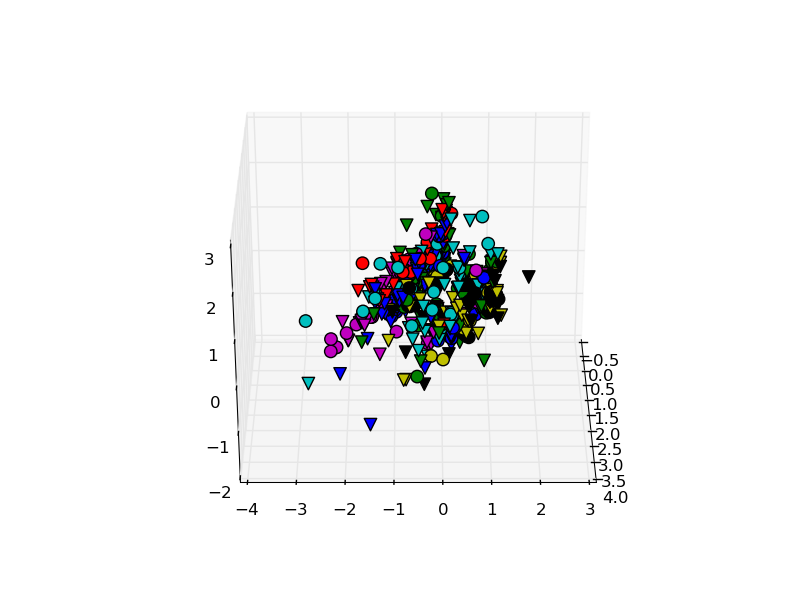
\includegraphics[width=0.5\textwidth]{img/ej1_sanger_01_20}
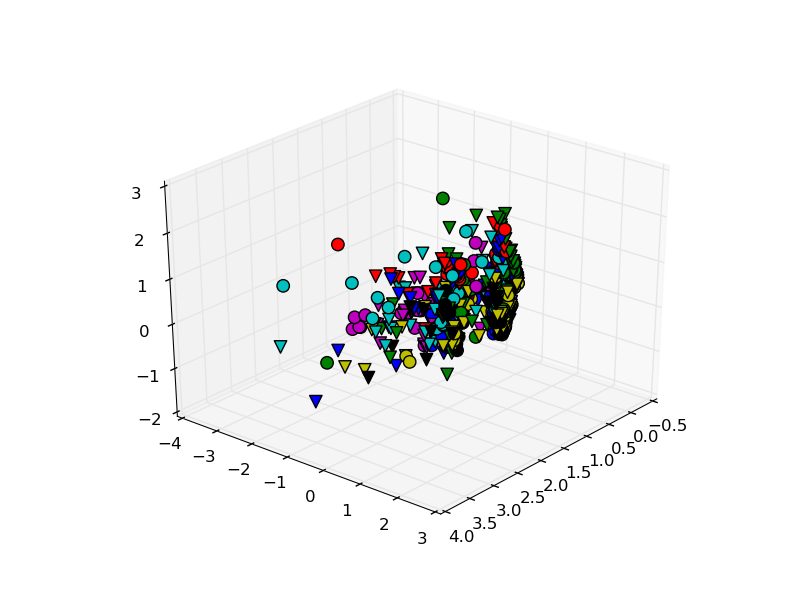
\includegraphics[width=0.5\textwidth]{img/ej1_sanger_01_40}
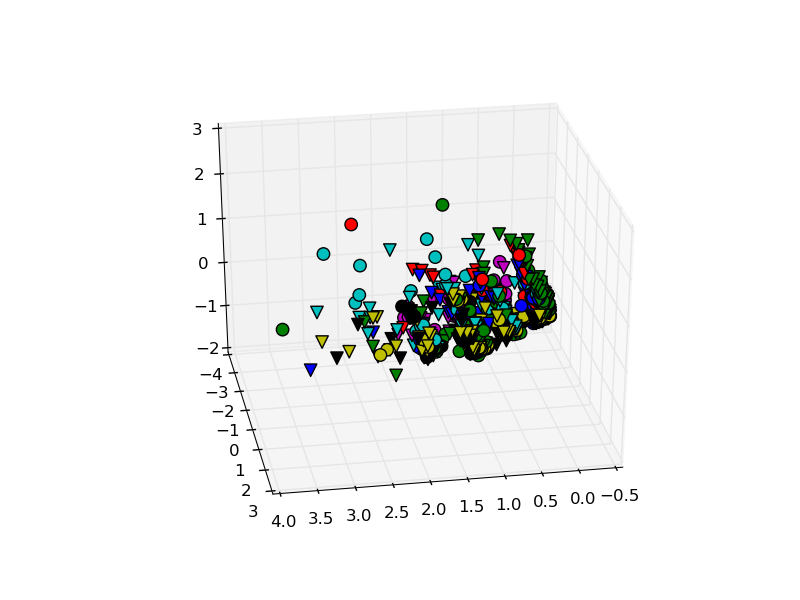
\includegraphics[width=0.5\textwidth]{img/ej1_sanger_01_80}
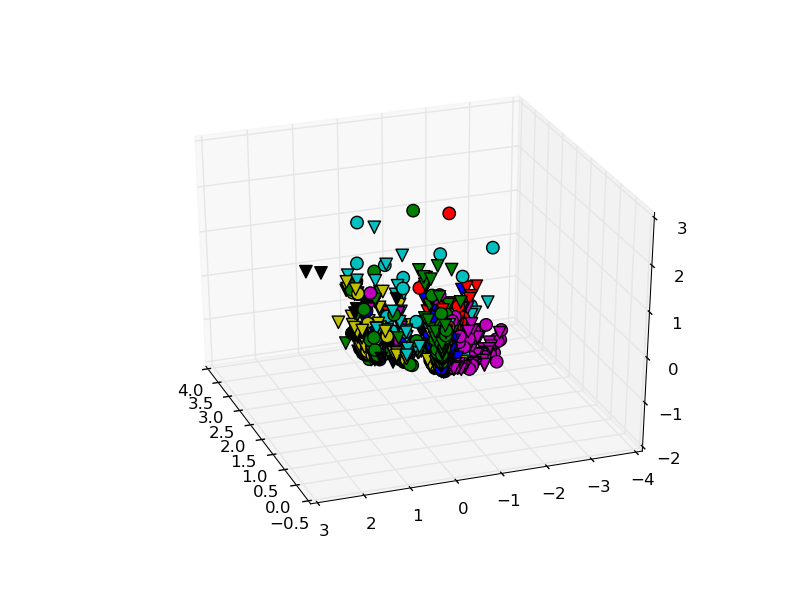
\includegraphics[width=0.5\textwidth]{img/ej1_sanger_01_160}
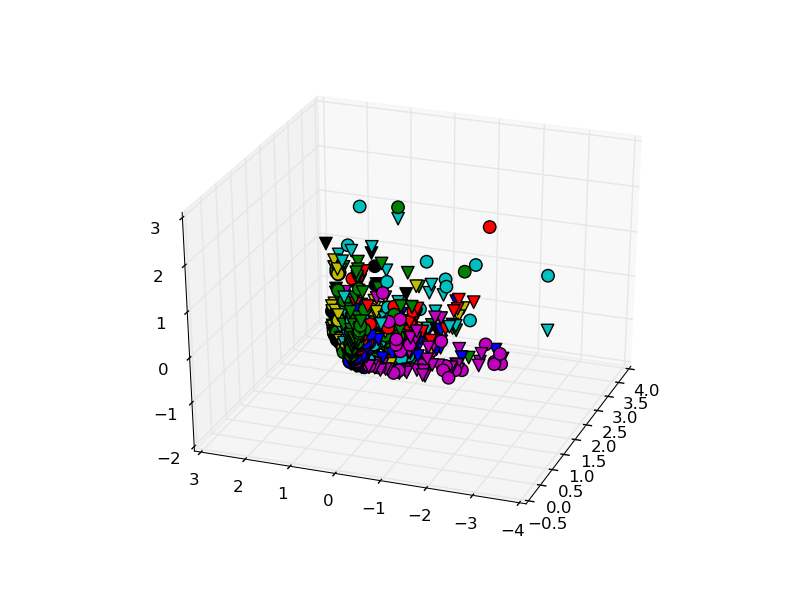
\includegraphics[width=0.5\textwidth]{img/ej1_sanger_01_200}
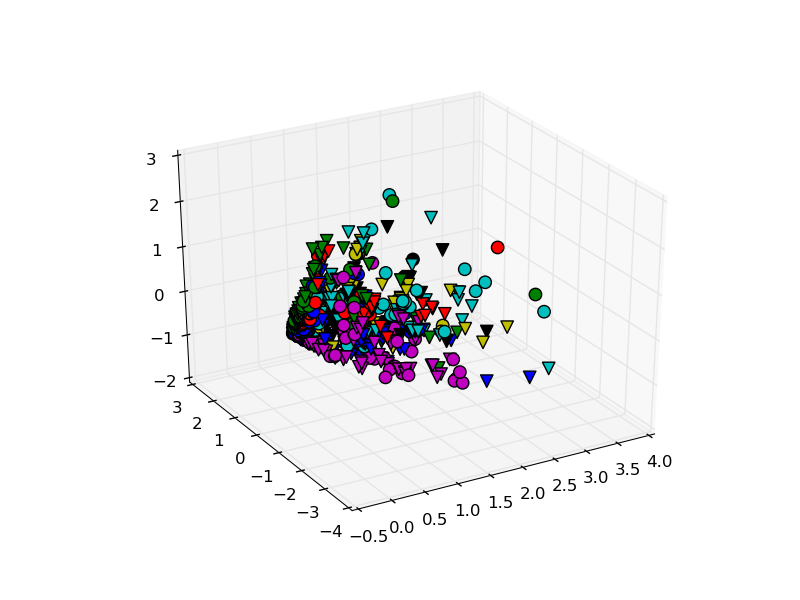
\includegraphics[width=0.5\textwidth]{img/ej1_sanger_01_240}


En este grafico lo que notamos muchos puntos estan dispersos, pero no solo dispersos, sino que son puntos dispersos de \textbf{distintos categorias}. 

Es dificil apreciar una agrupacion particular de un culor especifico, es decir, todos los colores estan un poco mezclados.

En particular el color amarillo se mezcla mucho con el verde, y el color rojo esta desparramado. 

Se nota tambien que el color violeta, al igual que el verde estan cerca de agruparse.

En algunos puntos se nota una mezcla intensa de color amarrilo y verde. Mientras que en otros lugares se nota esta mezcla pero de violeta, verde y azul.

Una particularidad de este grafico, es que el color rojo no resalta tanto y tiene un valor atipico.

con el mismo epsilon y con un learning rate de 0.001, en Oja obtuvimos 

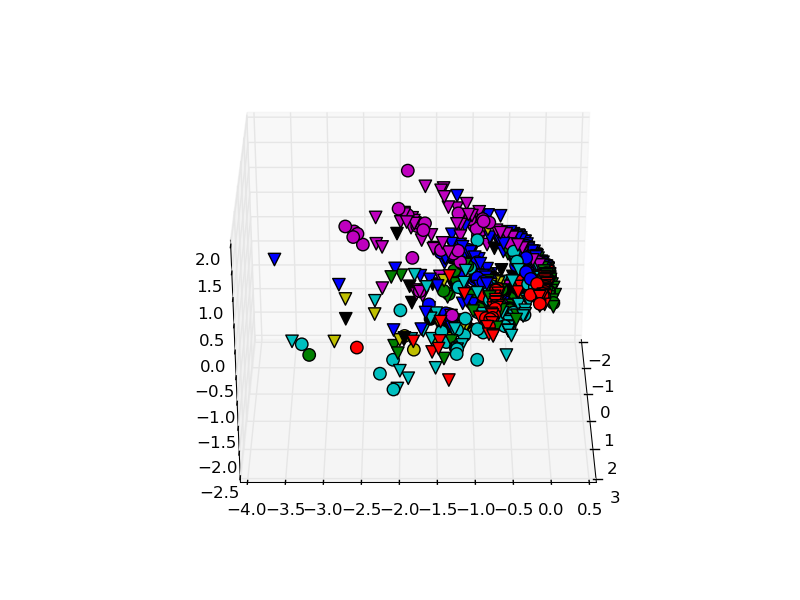
\includegraphics[width=0.5\textwidth]{img/ej1_oja_01_20}
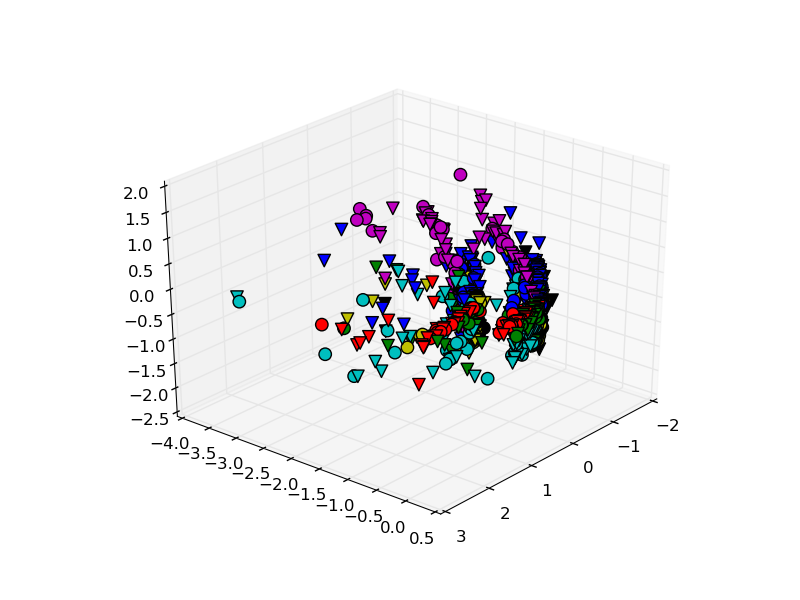
\includegraphics[width=0.5\textwidth]{img/ej1_oja_01_40}
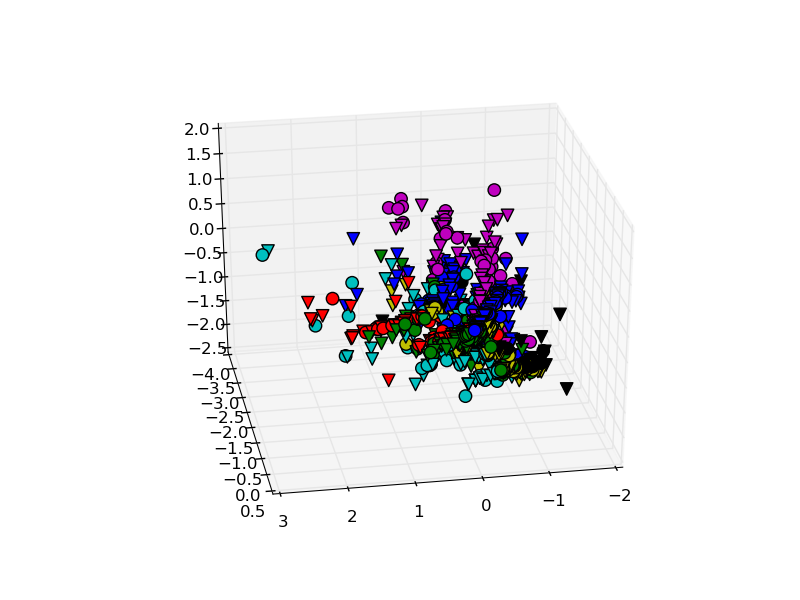
\includegraphics[width=0.5\textwidth]{img/ej1_oja_01_80}
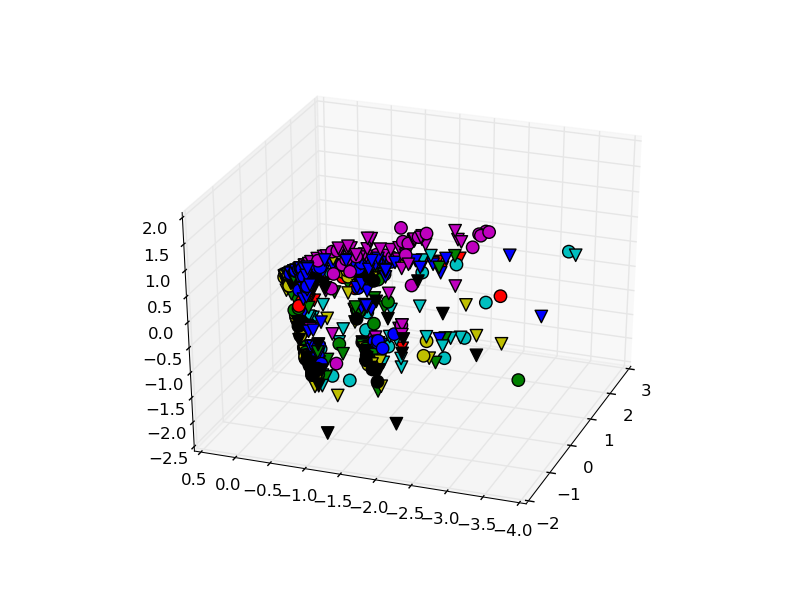
\includegraphics[width=0.5\textwidth]{img/ej1_oja_01_200}
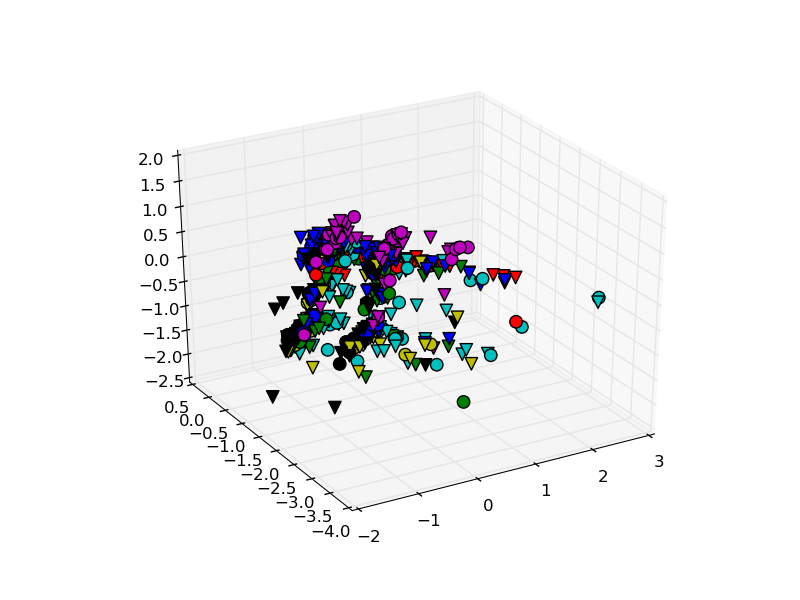
\includegraphics[width=0.5\textwidth]{img/ej1_oja_01_240}
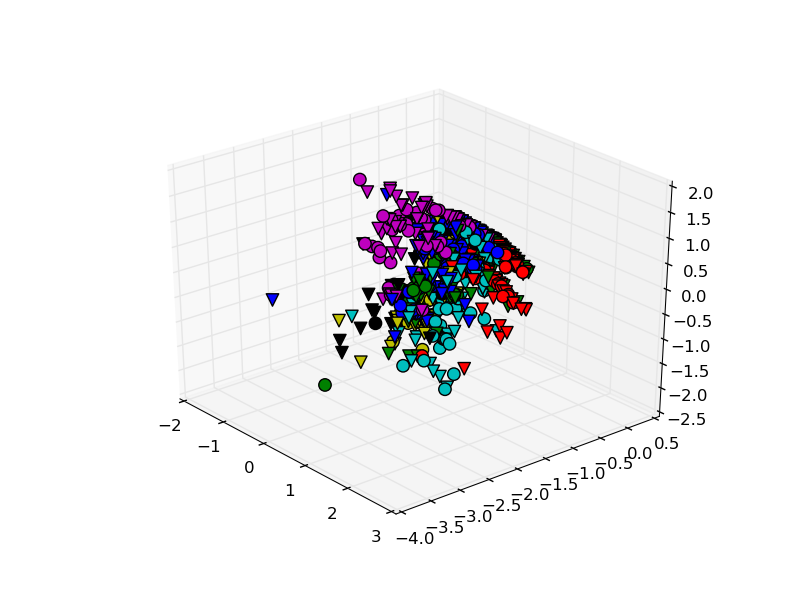
\includegraphics[width=0.5\textwidth]{img/ej1_oja_01_320}

En este grafico podemos observar donde grupos del mismoe lemento estan separados, como por ejemplo el violeta. Tambien observamos puntos outliers, dejando evidencia de que no llegaron a agruparse. 

En general se nota que las distintas categorias se mezclan intensamente y en casi ningun lado se llega a apreciar una categoria bien formada.

En algunas vistas (por ejemplo la ante ultima) vemos que no estan comprimidos, ni se nota una correlacion entre colores.

Como en la experimentacion anterior, se nota que tien mas problemas con el verde y el amarrillo que con el resto.


Por otro lado, analizando todos los graficos de las soluciones obtenidas deducimos que una mejora solucion (decision tomada analizando visualmente los graficos) es la siguiente:

Con un epsilon de 0.05 en sanger obtuvimos un grafico como el siguiente:


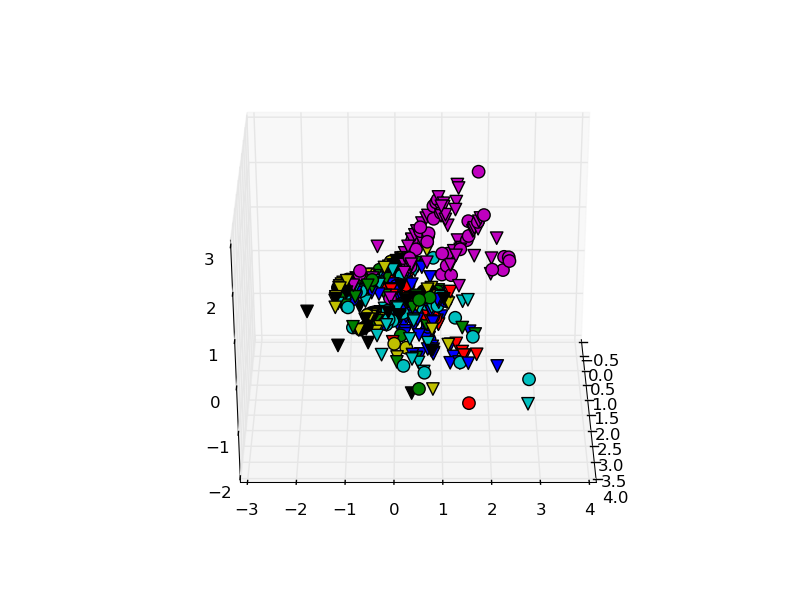
\includegraphics[width=0.5\textwidth]{img/ej1_sanger_005_20}
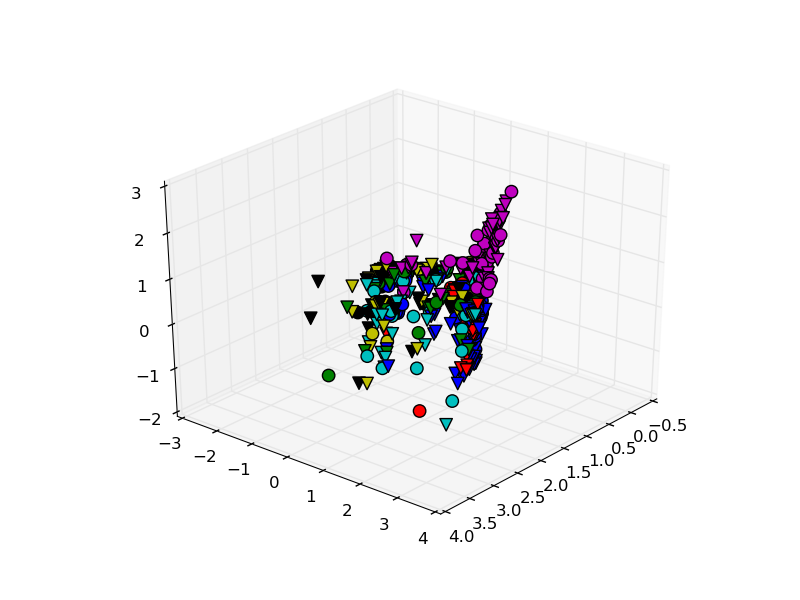
\includegraphics[width=0.5\textwidth]{img/ej1_sanger_005_40}
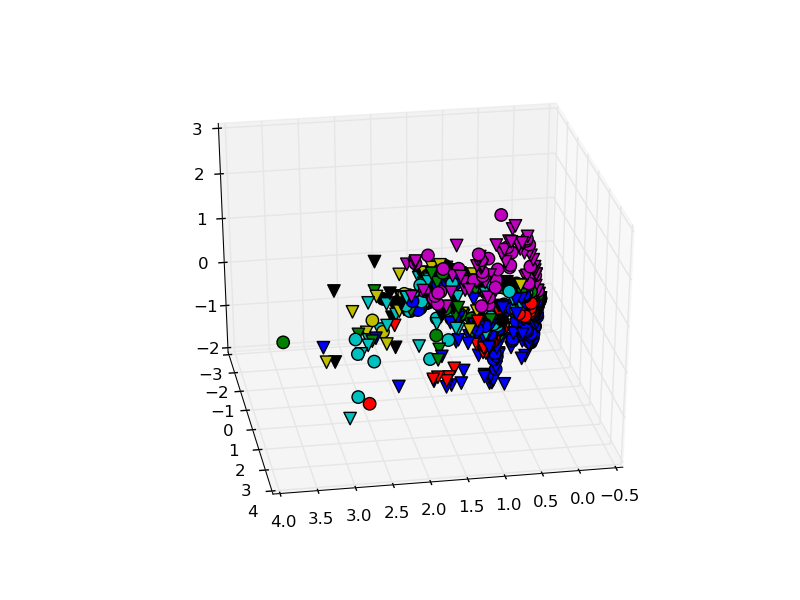
\includegraphics[width=0.5\textwidth]{img/ej1_sanger_005_80}
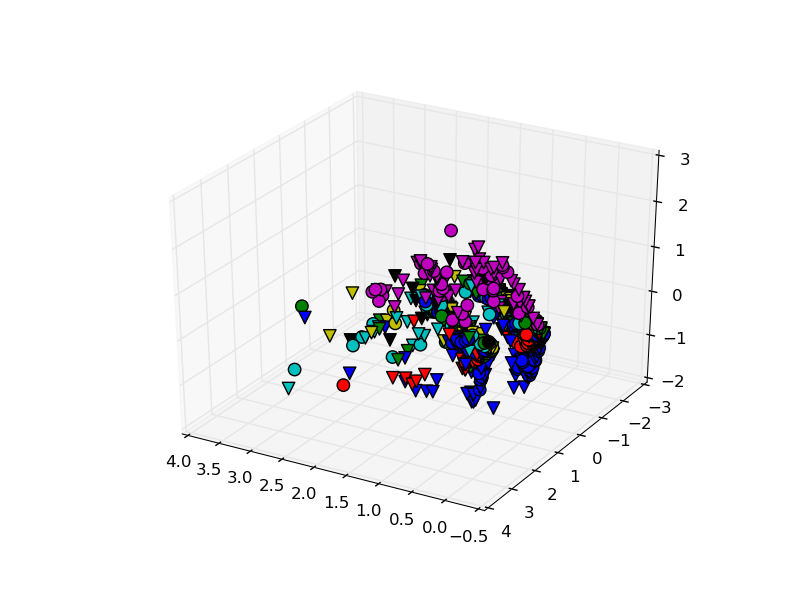
\includegraphics[width=0.5\textwidth]{img/ej1_sanger_005_120}
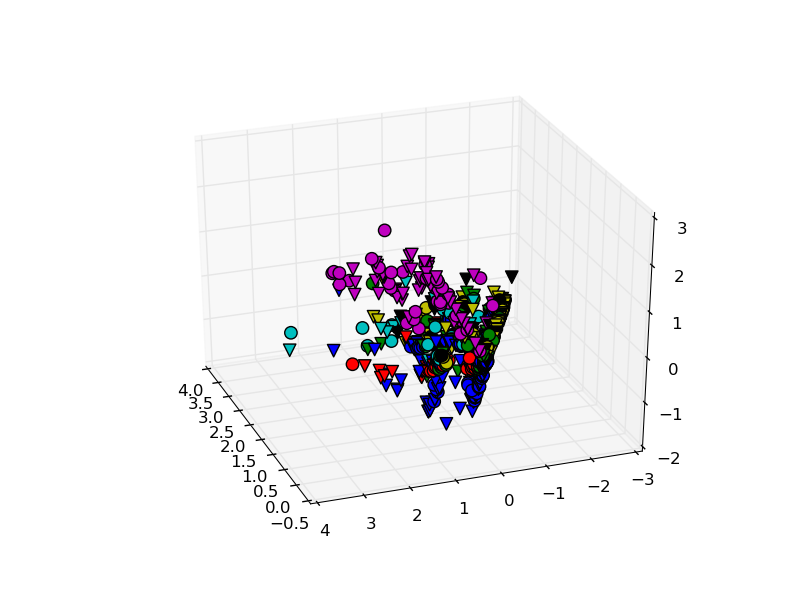
\includegraphics[width=0.5\textwidth]{img/ej1_sanger_005_160}
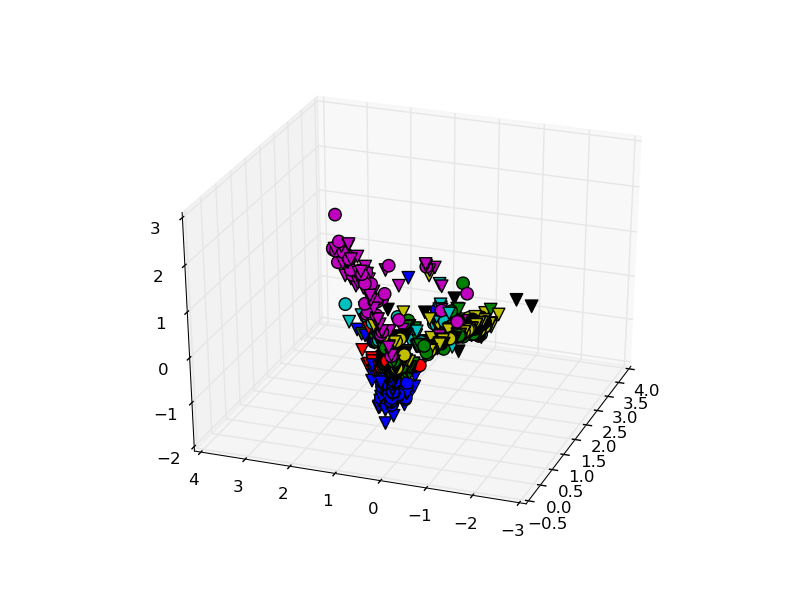
\includegraphics[width=0.5\textwidth]{img/ej1_sanger_005_200}


En estos graficos notamos claramente que el color violeta se separa en una categoria bien definida. 

Por otro lado, en estos graficos, a diferencia de los anteriores, se puede notar como el color azul tambien esta definiendo mejor la discretizacion que en experimentos anteriores.

En el ultimo grafico podems notar claramente la semaparacion entre el violeta y el azul, pero de igual manera vemos que el verde y amarrillo siguen mezclados, por suerte, no tanto como antes, pero siguen mezclando.

Con un epsilon de 0.05 y un Learning Rate de 0.001 en Oja obtuvimos:

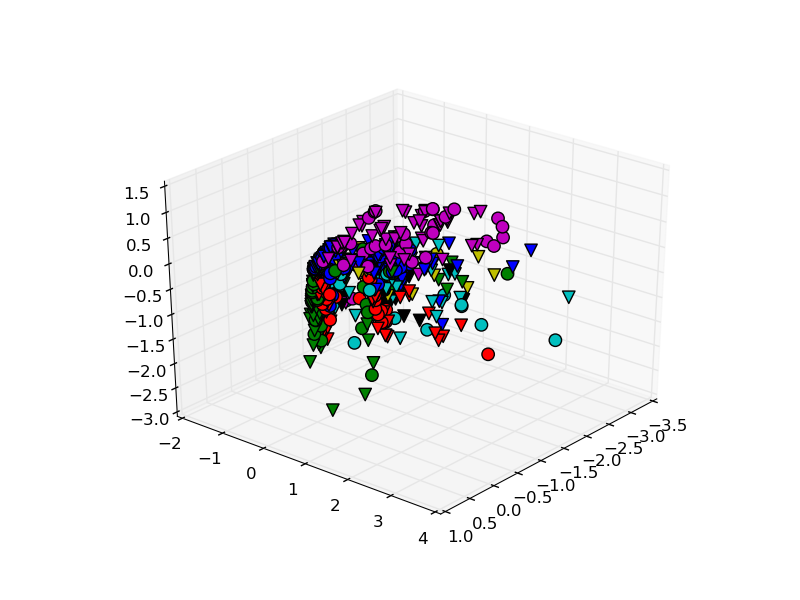
\includegraphics[width=0.5\textwidth]{img/ej1_oja_005_20}
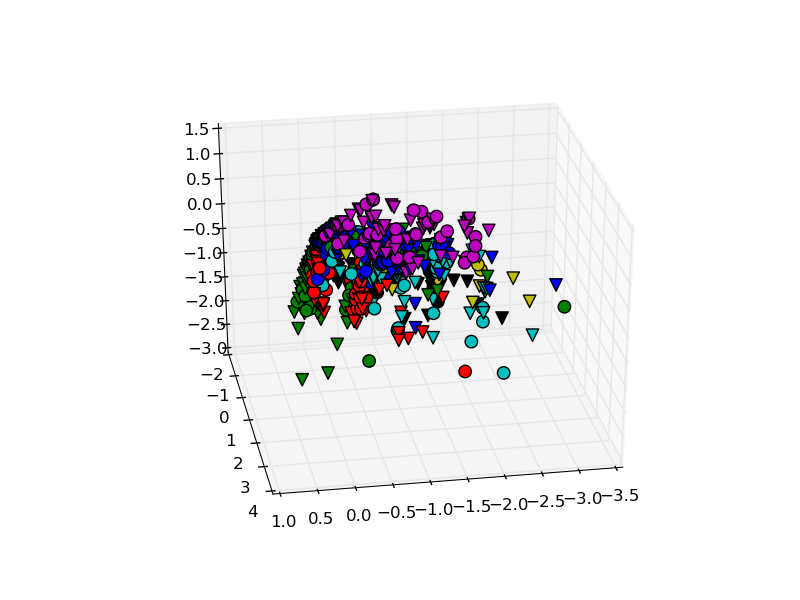
\includegraphics[width=0.5\textwidth]{img/ej1_oja_005_80}
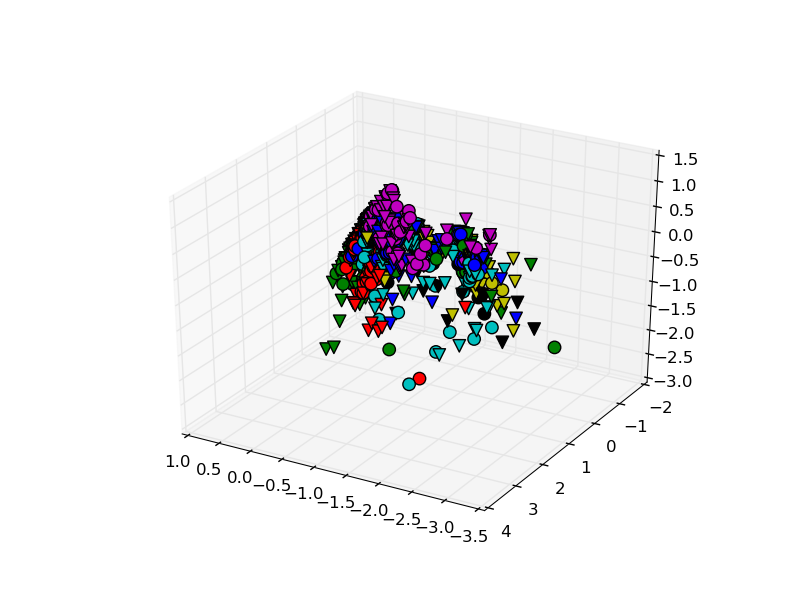
\includegraphics[width=0.5\textwidth]{img/ej1_oja_005_120}
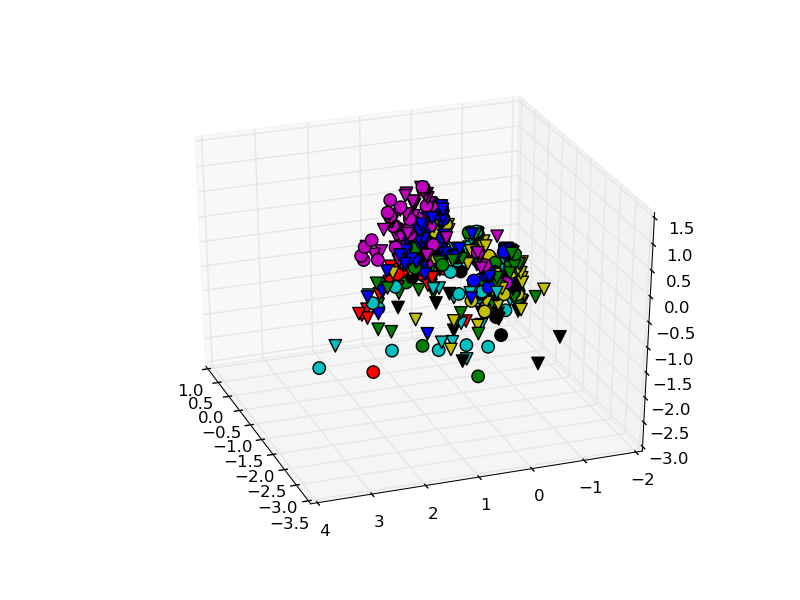
\includegraphics[width=0.5\textwidth]{img/ej1_oja_005_160}
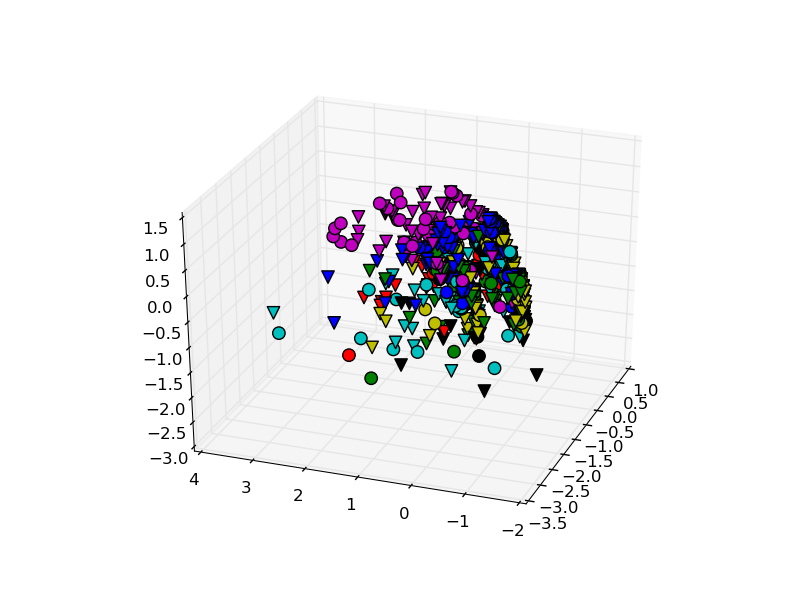
\includegraphics[width=0.5\textwidth]{img/ej1_oja_005_200}
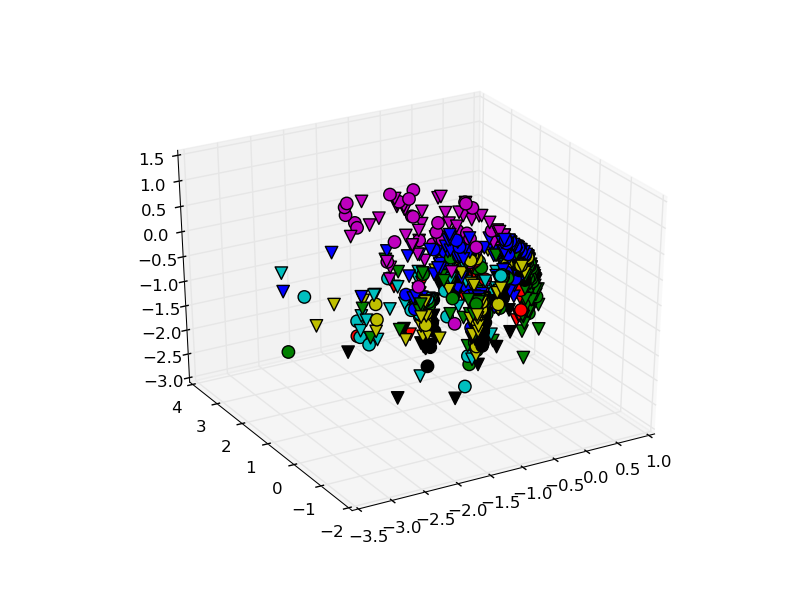
\includegraphics[width=0.5\textwidth]{img/ej1_oja_005_240}

En este grafico vemos, como en el anterior que el color violeta se agrupa de forma correcta.

Del mismo modo que el color azul. Lo mas notable de este grafico es que el color rojo empieza a aparecer en una especie de \textbf{categorizacion}, detalle que antes no pasaba. 

Otro factor importante es que el color verde y el amarillo no se mezclan tanto como en graficos anteriores.

\subsubsection{Conclusion}

Luego de analizar los graficos y resultados del ejercicio 1, podemos concluir que al contraio de lo que esperabamos, en lugar de agruparse en distintas esferas bien definidas, los resultados dieron mas heterogeneos.

Concluimos que la mejor solucion la ultima de Oja (epsilon: 0.05 y learning rate: 0.001) esto es debido a las justificaciones explicadas previamente. En general, se notan las categorias mejor agrupadas.

En general, notamos que los graficos poseen unas lineas de colores bien definidas, esto es, asumiendo que las categorias son ortoganles, porque cada categoria trata de ajustarce a una dimension, y al haber 9 categorias no alcanzan lsa dimenseiones, por lo tanto vemos estos solapamientos.

\subsection{Ejercicio 2}

Para el ejercicio 2 implementamos un algoritmo para probar lsa diferentes combinaciones de epocas, las cuales influyen en el sigma y distintos tamaños de salida. Para cada uno de estas variamos el Learning Rate y guardamos los graficos resultantes.

Una vez conseguidos todos los graficos hicimos un analisis observando cual tiene una mejor agrupacion, al igual que en el ejercicio 1, pero esta vez en el plano.


\begin{lstlisting}[caption=pruebas]
	
def prueba():
	file="tp2_training_dataset.csv"
	train_data = np.genfromtxt(file, delimiter=',',usecols=range(1,857))
	train_data=train_data[:600]
	test_data  = np.genfromtxt(file, delimiter=',',usecols=range(0,857))
	if not os.path.exists("imgs/ej2"):
		os.makedirs("imgs/ej2")
	sigma=0.001
	for epoca in [500,1000,1500]:
		for M in [3,5,9,20,30,40]:
			for lrate in np.linspace(0.001, 0.1, 20):
				red = som(M, M, lrate,sigma)
				red.train(train_data,epoca)
				img_name="imgs/ej2/train M "+str(M)+" lrate "+str(lrate)+" sigma"+str(sigma)+" 
				                                                    epocas "+str(epoca)+".jpg"
				graficador(red,test_data[:600],img_name)
				img_name="imgs/ej2/test M "+str(M)+" lrate "+str(lrate)+" sigma"+str(sigma)+" 
				                                                   epocas "+str(epoca)+".jpg"
				graficador(red,test_data[600:],img_name)

\end{lstlisting}

